\chapter{Fractional Step Method}
\label{FractionalStepM}
The equations to be solved are the conservation of mass and the conservation of momentum:
\begin{equation}
\begin{aligned}
\nabla\cdot\vec{v}=0 \\
\rho\frac{\partial\vec{v}}{\partial t}+\rho\left(\vec{v}\cdot\nabla\right)\vec{v}=-\nabla p+\mu\nabla^{2}\vec{v}
\end{aligned}
\end{equation}
According to the Helmholtz-Hodge theorem, it is possible to decompose any vector in a divergence-free vector parallel to the boundary and a gradient field, and this decomposition is unique \cite{CTTC}.

Assuming constant density and viscosity, the convective and viscosity terms can be grouped together in a single variable $R\left(\vec{v}\right)$, rewriting the Navier-Stokes equation as:
\begin{equation}
\rho\frac{\partial\vec{v}}{\partial t}=R\left(\vec{v}\right)-\nabla p
\label{RNSFSM}
\end{equation}
where $R\left(\vec{v}\right)=-\rho\left(\vec{v}\cdot\nabla\right)\vec{v}+\mu\nabla^{2}\vec{v}$.
Integrating the equation \ref{RNSFSM} over time:
\begin{equation}
\rho\frac{\vec{v}^{n+1}-\vec{v}^{n}}{\Delta t}=R^{n+\frac{1}{2}}\left(\vec{v}\right)-\nabla p^{n+1}
\end{equation}
However, the term $R^{n+\frac{1}{2}}\left(\vec{v}\right)$ is not easy to evaluate. To do so, the Adams-Bashforth second-order scheme is used:
\begin{equation}
R^{n+\frac{1}{2}}\left(\vec{v}\right)\approx\frac{3}{2}R\left(\vec{v^{n}}\right)-\frac{1}{2}R\left(\vec{v}^{n-1}\right)
\label{AdamsBashforth}
\end{equation}
Applying the Helmholtz-Hodge Theorem, the intermediate velocity is easily obtained:
\begin{equation}
\vec{v}^{P}=\vec{v}^{n+1}+\frac{\Delta t}{\rho}\nabla p^{n+1}
\label{IntermediateVelocity}
\end{equation}
Introducing this expression to the integrated equation:
\begin{equation}
\rho\frac{\vec{v}^{P}-\vec{v}^{n}}{\Delta t}=R^{n+\frac{1}{2}}\left(\vec{v}\right)
\label{IntermediatewithR}
\end{equation}
And finally, applying the divergence to the expression of the intermediate velocity $\vec{v}^{P}$ \ref{IntermediateVelocity}, the Poisson equation is obtained:
\begin{equation}
\nabla\cdot\vec{v}=\frac{\Delta t}{\rho}\nabla^{2}p
\label{Poisson}
\end{equation}

\section{Fractional Step Method algorithm}
With all these expressions the fractional step method (FSM) can be finally implemented, following the next scheme:
\begin{enumerate}
	\item Evaluate $R^{n+\frac{1}{2}}\left(\vec{v}\right)$.
	\item Calculate the intermediate velocity with equation \ref{IntermediatewithR}.
	\item Calculate the pressure $p^{n+1}$ from the Poisson equation \ref{Poisson} using a linear solver.
	\item Calculate the velocity at the next time step with equation \ref{IntermediateVelocity}.
\end{enumerate}
However, the FSM can be problematic if the mesh of the problem is not correctly implemented. To avoid having solutions with no physical sense, it is important to use staggered meshes or collocated meshes. The discretization of the domain as well as a further explanation of the described steps are going to be developed in the following sections.

\section{Discretization}
\label{FSMDiscretization}
To avoid convergence problems or incorrect solutions (checkerboard problem), the staggered meshes are used. As shown in figure \ref{staggered}, in a two-dimensional case there are 3 control volumes, one for each variable: $p_{P}$, $u_{P}$ and $v_{P}$. They are coloured in black, red and green respectively. The black dots are the nodes in which the pressure is calculated, the red arrows are the nodes of the horizontal velocity, and the green arrows are the nodes of the vertical velocity.
\begin{figure}
	\centering
	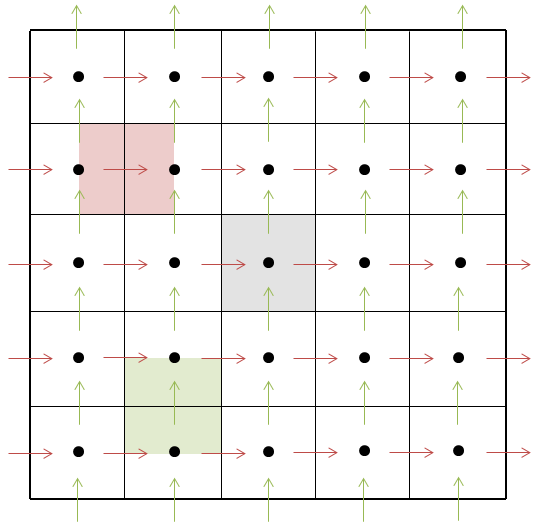
\includegraphics[scale=0.65]{DrivenCavity/staggered}
	\caption{Staggered meshes (2D)}
	\label{staggered}
\end{figure}

\subsection{Intermediate velocity discretization}
First of all, it is necessary to discretize the expression of R of the equation \ref{RNSFSM}:
\begin{equation}
R\left(\vec{v}\right)=-\rho\left(\vec{v}\cdot\nabla\right)\vec{v}+\mu\nabla^{2}\vec{v}
\end{equation}
This variable is a vector. Integrating the expression over the control volume of the horizontal velocity staggered mesh in the horizontal direction:
\begin{equation}
\int_{\Omega_{x}}R\left(u\right)d\Omega_{x}=-\int_{\Omega_{x}}\left(\rho\vec{v}\cdot\nabla\right)ud\Omega_{x}+\int_{\Omega_{x}}\mu\nabla^{2}ud\Omega_{x}
\end{equation}
Now, applying the Gauss Theorem:
\begin{equation}
R\left(u\right)V_{P}=-\int_{\partial\Omega_{x}}\left(\rho\vec{v}\right)u\cdot\vec{n}dS+\int_{\partial\Omega_{x}}\mu\nabla u\cdot\vec{n}dS
\end{equation}
The final integration of R in the horizontal direction results as:
\begin{multline}
R\left(u\right)V_{P}=\left[\mu_{e}\frac{u_{E}-u_{P}}{d_{EP}}A_{e}+\mu_{n}\frac{u_{N}-u_{P}}{d_{NP}}A_{n}-\mu_{w}\frac{u_{P}-u_{W}}{d_{WP}}A_{w}-\mu_{s}\frac{u_{P}-u_{S}}{d_{SP}}A_{s}\right] \\
-\left[\left(\rho u\right)_{e}u_{e}A_{e}+\left(\rho v\right)_{n}u_{n}A_{n}-\left(\rho u\right)_{w}u_{w}A_{w}-\left(\rho v\right)_{s}u_{s}A_{s}\right]
\end{multline}
The same approach is used in the vertical direction, obtaining the following expression:
\begin{multline}
	R\left(v\right)V_{P}=\left[\mu_{e}\frac{v_{E}-v_{P}}{d_{EP}}A_{e}+\mu_{n}\frac{v_{N}-v_{P}}{d_{NP}}A_{n}-\mu_{w}\frac{v_{P}-v_{W}}{d_{WP}}A_{w}-\mu_{s}\frac{v_{P}-v_{S}}{d_{SP}}A_{s}\right] \\
	-\left[\left(\rho u\right)_{e}v_{e}A_{e}+\left(\rho v\right)_{n}v_{n}A_{n}-\left(\rho u\right)_{w}v_{w}A_{w}-\left(\rho v\right)_{s}v_{s}A_{s}\right]
\end{multline}

The main problem of these expressions is the evaluation of the velocities and the mass flows in the faces of the control volume. To calculate the velocities in the faces some of the numerical schemes previously discussed are used: CDS, UDS... In the case of the mass flows per surface unit, the staggered meshes have to be taken into account:
\begin{figure}[h]
	\centering
	\begin{minipage}{.5\textwidth}
		\centering
		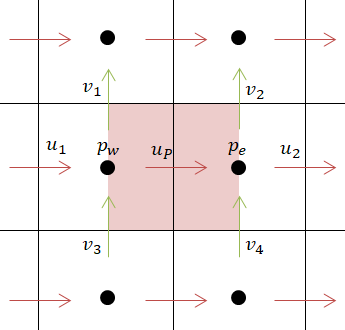
\includegraphics[scale=0.7]{DrivenCavity/mflowx3}
		\caption{Control volume of the horizontal velocity}
		\label{DCmflowx}
	\end{minipage}%
	\begin{minipage}{.5\textwidth}
		\centering
		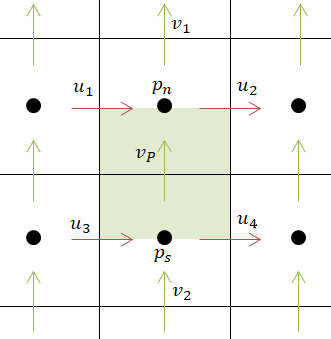
\includegraphics[scale=0.68]{DrivenCavity/mflowy3}
		\caption{Control volume of the vertical velocity}
		\label{DCmflowy}
	\end{minipage}
\end{figure}
\begin{itemize}
	\item The calculation of the mass flow per surface unit in the control volume of the horizontal velocity \ref{DCmflowx} is simple in the case of the horizontal mass flows:
	\begin{equation}
	\left(\rho u\right)_{e}=\frac{\rho u_{P}+\rho u_{2}}{2}
	\end{equation}
	\begin{equation}
	\left(\rho u\right)_{w}=\frac{\rho u_{1}+\rho u_{P}}{2}
	\end{equation}
	But the vertical flows are somehow more difficult:
	\begin{equation}
	\left(\rho v\right)_{n}=\frac{\rho v_{1}+\rho v_{2}}{2}
	\end{equation}
	\begin{equation}
	\left(\rho v\right)_{s}=\frac{\rho v_{3}+\rho v_{4}}{2}
	\end{equation}
	\item The calculation of the mass flow per surface unit in the control volume of the vertical velocity \ref{DCmflowy} is similar to that of the horizontal velocity. Starting with the horizontal flows:
	\begin{equation}
	\left(\rho u\right)_{e}=\frac{\rho u_{2}+\rho u_{4}}{2}
	\end{equation}
	\begin{equation}
	\left(\rho u\right)_{w}=\frac{\rho u_{1}+\rho u_{3}}{2}
	\end{equation}
	And the vertical ones:
	\begin{equation}
	\left(\rho v\right)_{n}=\frac{\rho v_{1}+\rho v_{P}}{2}
	\end{equation}
	\begin{equation}
	\left(\rho v\right)_{s}=\frac{\rho v_{P}+\rho v_{2}}{2}
	\end{equation}
\end{itemize}
Once the value of R is calculated using the expressions developed above and the Adams-Bashforth scheme \ref{AdamsBashforth}, the intermediate velocity can be computed rearranging the equation \ref{IntermediatewithR}:
\begin{equation}
\vec{v}^{P}=\vec{v}^{n}+\frac{\Delta t}{\rho}R^{n+\frac{1}{2}}\left(\vec{v}\right)
\end{equation}

\subsection{Pressure discretization}
The next step is to obtain the pressure in the next time step with the Poisson equation. Knowing the space discretization of the domain, the discretized Poisson equation can be calculated. Integrating the expression \ref{Poisson} over the domain and applying the divergence theorem, the following expression can be easily obtained:
\begin{equation}
\begin{aligned}
\frac{p_{E}^{n+1}-p_{P}^{n+1}}{d_{EP}}A_{e}+\frac{p_{N}^{n+1}-p_{P}^{n+1}}{d_{NP}}A_{n}-\frac{p_{P}^{n+1}-p_{W}^{n+1}}{d_{WP}}A_{w}-\frac{p_{P}^{n+1}-p_{S}^{n+1}}{d_{SP}}A_{s}= \\
\frac{1}{\Delta t}\left[\left(\rho u^{P}\right)_{e}A_{e}+\left(\rho v^{P}\right)_{n}A_{n}-\left(\rho u^{P}\right)_{w}A_{w}-\left(\rho v^{P}\right)_{s}A_{s}\right]
\end{aligned}
\end{equation}
Rewriting the equation using discretization coefficients:
\begin{equation}
a_{P}p_{P}^{n+1}=a_{E}p_{E}^{n+1}+a_{W}p_{W}^{n+1}+a_{N}p_{N}^{n+1}+a_{S}p_{S}^{n+1}+b_{P}
\end{equation}
where
\begin{equation}
a_{P}=a_{E}+a_{W}+a_{N}+a_{S}
\end{equation}
\begin{equation}
a_{E}=\frac{A_{e}}{d_{EP}}
\end{equation}
\begin{equation}
a_{W}=\frac{A_{w}}{d_{WP}}
\end{equation}
\begin{equation}
a_{N}=\frac{A_{n}}{d_{NP}}
\end{equation}
\begin{equation}
a_{S}=\frac{A_{s}}{d_{SP}}
\end{equation}
\begin{equation}
b_{P}=-\frac{1}{\Delta t}\left[\left(\rho u^{P}\right)_{e}A_{e}+\left(\rho v^{P}\right)_{n}A_{n}-\left(\rho u^{P}\right)_{w}A_{w}-\left(\rho v^{P}\right)_{s}A_{s}\right]
\end{equation}

\subsection{Velocity discretization}
With the equation \ref{IntermediateVelocity} the horizontal and vertical velocities at the next time step can be calculated:
\begin{equation}
u_{P}^{n+1}=u_{P}^{P}-\frac{\Delta t}{\rho}\frac{p_{e}^{n+1}-p_{w}^{n+1}}{d_{ew}}
\end{equation}
\begin{equation}
v_{P}^{n+1}=v_{P}^{P}-\frac{\Delta t}{\rho}\frac{p_{n}^{n+1}-p_{s}^{n+1}}{d_{ns}}
\end{equation}

\section{Time step}
The fractional step method is an explicit method. In order to obtain accuracy in the results, the time step has to be correctly chosen. To do so, it is recalculated in each iteration of the algorithm using a Courant-Friedrich-Levy (CFL) condition. Two time steps are defined, one of them depends on the convective term and the other one on the diffusive term:
\begin{equation}
\Delta t_{c}=\min\left(0.35\frac{\Delta x}{|v|}\right)
\end{equation}
\begin{equation}
\Delta t_{d}=\min\left(0.20\frac{\rho\left(\Delta x\right)^{2}}{\mu}\right)
\end{equation}
If the mesh, the density and the viscosity are constant, the time step defined by the diffusive term is constant, so it only has to be calculated at the beginning of the simulation, as it depends on the velocity. But the time step given by the convective term changes with each iteration. The final time step that is going to be used is the smallest one:
\begin{equation}
\Delta t=\min\left(\Delta t_{c}, \Delta t_{d}\right)
\end{equation}